\setcounter{chapter}{13-1}

\chapter{Autoencoders}

    Through neural networks, we've \textbf{upgraded} the set of models we can use to do classification and regression tasks.

    \begin{itemize}
        \item Neural networks become more complex and \textbf{expressive} as we add more \textbf{layers}.
    \end{itemize}

    We'll spend the next few chapters exploring NNs: creating new variants (CNNs, RNNs), for example.
    
    In this chapter, we'll investigate a different kind of application: \orgg{autoencoders.}

    \subsection{Unsupervised Learning}

        In chapter 6, we discussed an \gren{unsupervised} learning problem: clustering.

        \begin{itemize}
            \item Classification tells us which classes to use. By contrast, clustering \textbf{doesn't} "know" the classes we're looking for.

            \begin{itemize}
                \item Instead, we discover new classes ("clusters"), using the $k$-means algorithm.
            \end{itemize}
            
            \item This lack of guidance is what makes clustering \textbf{unsupervised}.
        \end{itemize}

        Clustering was used as a form of \textbf{data analysis}: we were able to learn more about the \textbf{structure} of our data, by finding what sorts of "groups" existed.

        We'll use autoencoders for a different task, that follows the same theme: learning more about the data, by attempting to look for an \textbf{unknown solution} to a simple problem.

    \subsection{Autoencoders: Compression}

        This time, our problem is not cluster-finding, but instead, \orgg{compression}. We want to take our input data, and find a more \textbf{space-efficient} way to represent it.

        Typically, this means reducing the number of \textbf{dimensions}/variables. 

        \begin{itemize}
            \item \miniex turning a 10-dim data point into a 4-dim data point.
        \end{itemize}

        Why would we do this? Because of what we gain from this task:

        \begin{itemize}
            \item A good compression algorithm should be able to be \textbf{decompressed}, while keeping the result mostly similar.
                \begin{itemize}
                    \item That means that our compression must preserve \textbf{essential} information, so it's possible to retrieve later.
                \end{itemize}

            \item By observing what's the algorithm decides to preserve and discard, can teach us what matters, and what doesn't.\\
        \end{itemize}

        \begin{concept}
            Learning a \vocab{compression algorithm} for your dataset creates a \gren{simplified} representation, that still keeps the most important, distinct information.

            Based on the information we find in that representation, we can figure out what components were "\purp{important}".
        \end{concept}
        
        Our compression/decompression system needs to do two things:

        \begin{itemize}
            \item \gren{Reproduce} the original data well
            \item Do so in a way that lets us \gren{distinguish} one data point from another
        \end{itemize}

        Based on this, a trained autoencoder can provide us some unexpected insights.

        \subsecdiv

        We can better see this with an example.

        \miniex Consider a database of human faces.

        \begin{itemize}
            \item It's more space-efficient if you can just re-use a "\textbf{template}" for a face, and just modify it.
                \begin{itemize}
                    \item So, your model might memorize what a face "generally" looks like.
                    \item That way, it doesn't have to waste space in the compression for data that appears frequently.
                \end{itemize}
                
            \item Then, your compressed data only needs to store what's special, or different, about the face it represents.

                \begin{itemize}
                    \item So, you learn what separates different faces from each other, based on the info in the compressed model.
                \end{itemize}
        \end{itemize}

    \subsection{Training}

        This representation might even be easier for a new model to \textbf{train} with: 

            \begin{itemize}
                \item We've omitted some unnecessary information that can \textbf{distract} our model.
                    \note{The model can overfit to \textbf{noise} in these extra variables.}
                \item With a simpler input, it's faster to train, and compute answers.\\
            \end{itemize}

            \begin{concept}
                Just like how \purp{clustering} is used to improve downstream tasks, \gren{compression} can be, too.

                Compressing your input can improve learning, so it takes less data to train.
            \end{concept}

            \phantom{}

            \begin{clarification}
                Not all compression is created equal!

                Auto-encoding compresses in a way that contains \gren{relevant information}.

                \subsecdiv

                However, in the Feature representation chapter, we discussed \vocab{binary code}: representing a number in \textbf{binary}, because it requires fewer features.

                \begin{itemize}
                    \item This kind of compression doesn't emphasize what's "important" about the feature representation.
                \end{itemize}

                Binary compression is \redd{worse}, not better! Instead of isolating useful information, it \redd{obscures} it, forcing the model to learn binary.
            \end{clarification}


        


\pagebreak
\section{Autoencoder Structure}

    \subsection{Visualization}

        Our encoder is a \textbf{compression} algorithm, which takes an input $\ex{x}{i}$, and returns a new "transformed" input $\ex{a}{i}$, with a lower dimensionality.
            \note{Note: you don't have to take the vectors in equation \textbf{8.1} literally. 

            \phantom{}
            
            You're not \textbf{required} to have $\operatorname{Dimension}(a)>2$, as in \textbf{8.1}.}
    
        \begin{equation}
            \overbrace{
            \begin{bmatrix}
                x_1 \\ x_2 \\ x_3 \\ \vdots \\ x_d
            \end{bmatrix}
            \longrightarrow
            \begin{bmatrix}
                a_1 \\ a_2 \\ \vdots \\ a_k
            \end{bmatrix}
            }^{k < d}
        \end{equation}
    
        In other words, we're going from $x \in \RR^d$ to $a \in \RR^k$.
    
        \miniex Take the classic problem of the MNIST dataset: identifying the identity of a digit based on a 28 x 28 grid of pixels.

        \begin{figure}[H]
            \centering
            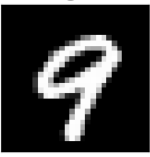
\includegraphics[width=30mm,scale=0.5]{images/autoencoder_images/mnist_9.png}
            \caption*{Here's an example of one data point: this represents the digit 9.}
        \end{figure}
    
        \begin{itemize}
            \item That means our input data has $784$ dimensions: $x \in \RR^{784}$.
                \note{Each pixel is actually \textbf{restricted} to $[0,255]$, but this statement is still technically true.}
    
            \item Below, we've used an encoder to compress it down to 2 dimensions: $a \in \RR^2$.
    
            \begin{equation}
                \begin{bmatrix}
                x_1 \\ x_2 \\  \vdots \\ x_{784}
                \end{bmatrix}
                \longrightarrow
                \begin{bmatrix}
                    a_1 \\ a_2 \\ 
                \end{bmatrix}
            \end{equation}
    
            \item The x-axis and y-axis indicate the two dimensions of our output, $a$.
        \end{itemize}
    
        \begin{figure}[H]
            \centering
            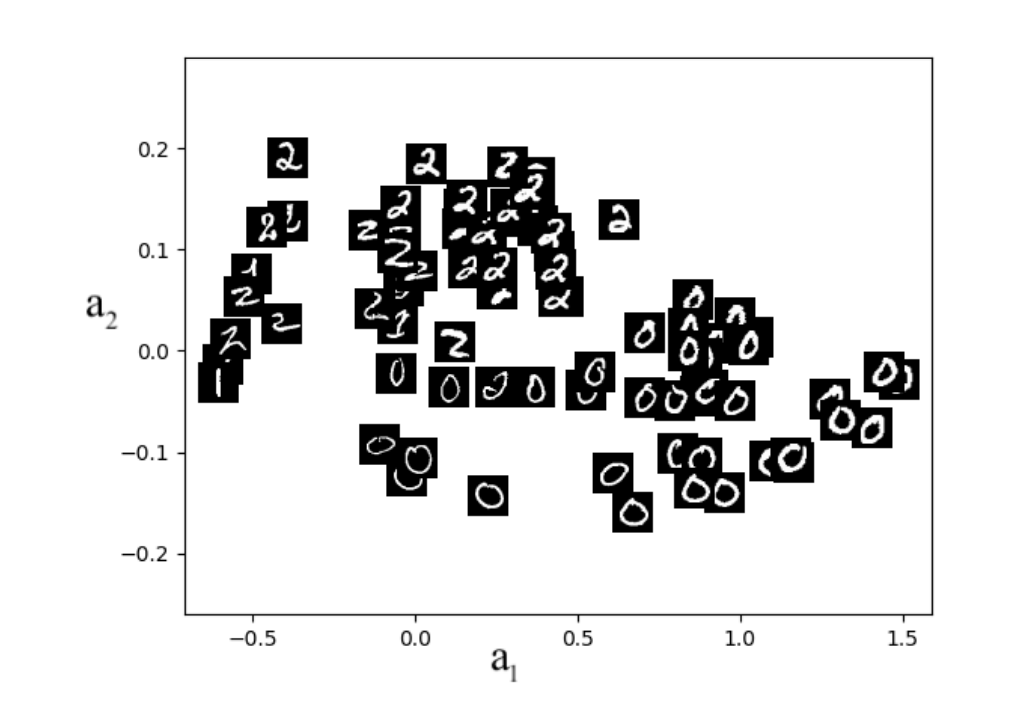
\includegraphics[width=70mm,scale=0.5]{images/autoencoder_images/mnist_compression.png}
            \caption*{Notice that digits with the same identity are near each other: our compressed representation seems to be storing some useful data about digits!}
        \end{figure}
    
        Somehow, we've created a \textbf{simplified} representation that, despite having only 2 variables, has a lot of useful information!

        \begin{itemize}
            \item With only a couple labelled data points, we could guess the digits of most of these pictures, based on how close they are.\\
        \end{itemize}

        \begin{clarification}
            This property, of "similar" data points, being \gren{close} in the latent space, is \redd{not} guaranteed, for any \purp{compressed representation} you create.

            However, it's a property we \textit{hope} to find, in a useful one.
        \end{clarification}

        But whether or not our data "organizes" nicely like this, we've still demonstrated another benefit of compression:

        \begin{itemize}
            \item It allows us to transform our data into a lower-dimensional, more \textbf{digestible} format.
            \item So, we can create better visualizations.\\
        \end{itemize}

    
        \begin{concept}
            One application of \orgg{compression} is using it for \gren{visualization}.
    
            A lower-dimensional version of a dataset is usually easier to diagram in a way humans can \gren{interpret} directly.

            \begin{itemize}
                \item Because this representation tends to be more \purp{dense} with information, it's often easier to draw useful conclusions.
            \end{itemize}
    
            It can also let us make simple predictions, or find patterns, since there are \purp{fewer} variables to pay attention to.
        \end{concept}


        This compressed version of data is called a "latent representation".\\

        \begin{definition}
            The \vocab{latent representation} of our data is the \purp{compressed} version, containing as much useful information as possible, with fewer variables.

            \begin{itemize}
                \item We call it \gren{latent} because original data $x$ is in a "hidden" form, but we can retrieve it by \textbf{decompressing}.
            \end{itemize}
            

            \subsecdiv

            The \vocab{latent space} represents all of the possible latent representations.
            \begin{itemize}
                \item This "space" follows the tradition of "input/feature spaces": sets with structure. In this case, the \purp{distance} between our data gives us the \purp{structure}.
            \end{itemize}

            Generally, a good latent space preserves \gren{information}: the reconstructed input still \textbf{communicates} what we were interested in, from the original input.
            
        \end{definition}

    \subsection{Anatomy of an Autoencoder}

        Our autoencoder's purpose is \textbf{compression}, but we need to make sure that this compression preserves the information that we want.\\

        \begin{definition}
            An \vocab{autoencoder} comes in two parts:

            \begin{itemize}
                \item An \purp{encoder}, which \purp{compresses} our ($d$-dim) input into the ($k$-dim) latent representation.

                \item A \gren{decoder}, which \gren{de-compresses} our latent representation, to try to re-create the input.
                    \begin{itemize}
                        \item This is used to make sure that our representation contains the information we need, to accurately re-construct the input.
                    \end{itemize}
            \end{itemize}

            The goals are:

            \begin{itemize}
                \item To create a \purp{smaller} latent representation, with dimensions $k < d$
                \item To make sure that this latent representation can \gren{accurately} re-construct our input
            \end{itemize}

            \subsecdiv

            \begin{itemize}
                \item The encoder and decoder can be any kind of function, but we will use \orgg{neural networks}.
            \end{itemize}
        \end{definition}

        This is where neural networks shine: with more powerful model class, we can do more complex math to create our "encoding".

        

    \subsection{One layer encoder/one layer decoder}

        For a simple demonstration, we'll use a version with a one-layer encoder and a one-layer decoder.

        We'll take our (\pur{$d$}-dim) input, and compress it into a (\grn{3}-dim) latent representation.

        \begin{itemize}
            \item Encoder: input $x \in \RR^d$, output (compressed) $a \in \RR^3$. 

                \begin{figure}[H]
                    \centering
                    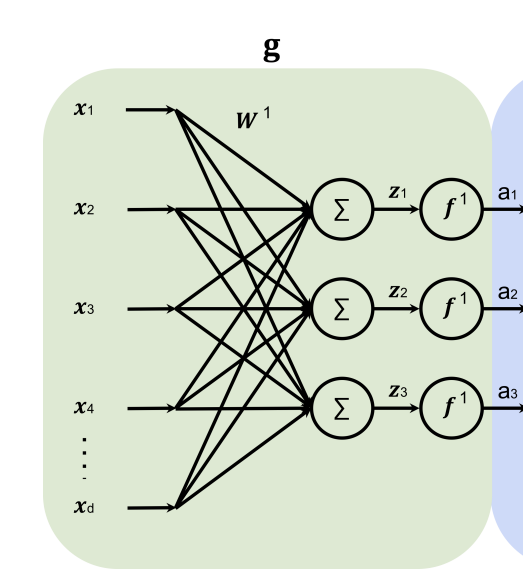
\includegraphics[width=40mm,scale=0.5]{images/autoencoder_images/encoder.png}
                \end{figure}
                    
            \item Decoder: input (compressed) $a \in \RR^3$, output (decompressed) $\tilde{x} \in \RR^d$.

                \begin{figure}[H]
                    \centering
                    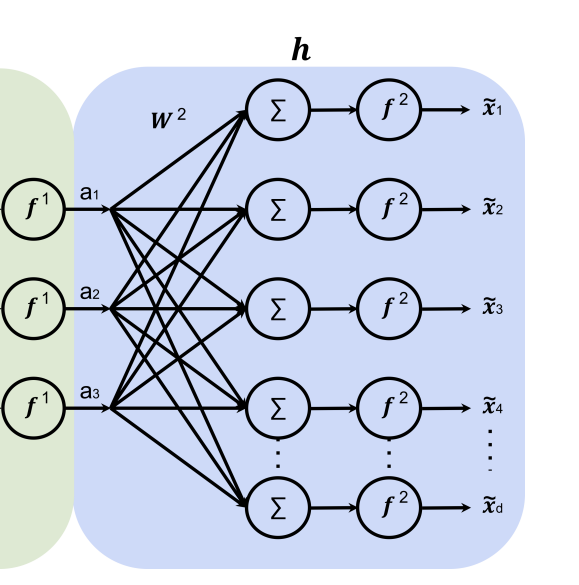
\includegraphics[width=40mm,scale=0.5]{images/autoencoder_images/decoder.png}
                \end{figure}
        \end{itemize}

        Taken together, we get our autoencoder:

        \begin{figure}[H]
            \centering
            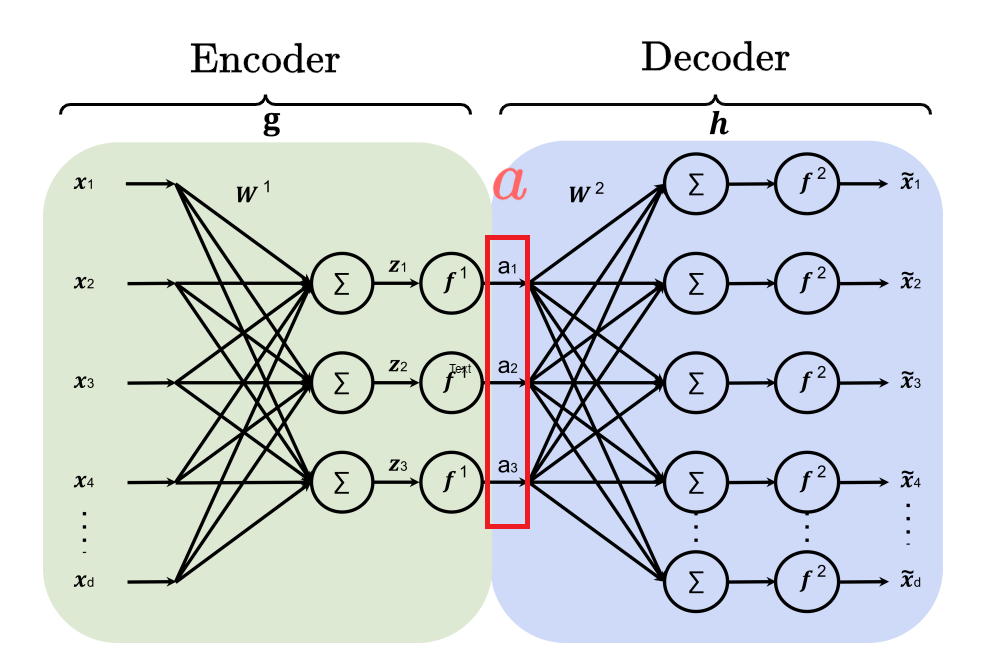
\includegraphics[width=90mm,scale=0.5]{images/autoencoder_images/encoder_decoder.png}

            \caption*{Note that, in addition to $W^1$ and $W^2$, we have a set of offsets that are not shown: $W^1_0$ and $W^2_0$.}
        \end{figure}

        Let's run through our network:

        \begin{itemize}
            \item The \gren{input} $x$ goes through the encoder network. This compresses into the \purp{latent representation} $a$.
                \begin{itemize}
                    \item $W^1$ has shape $(d \times k)$, or equivalently, $W^1 \in \RR^{d \times k}$
                    \item $W^1_0$ has shape $(k \times 1)$, or equivalently, $W^1_0 \in \RR^k$
                \end{itemize}

            \begin{equation}
                \org{z^1} = (W^1)^T \grn{x} + W^1_0 \qquad \qquad \red{a} = f(\org{z^1})
            \end{equation}

            \item The \purp{latent representation} goes through the decoder network. This de-compresses it into the \gren{re-constructed input}.
                \begin{itemize}
                    \item $W^2$ has shape $(k \times d)$, or equivalently, $W^2 \in \RR^{k \times d}$
                    \item $W^1_0$ has shape $(d \times 1)$, or equivalently, $W^2_0 \in \RR^d$
                \end{itemize}

                \begin{equation}
                \pur{z^2} = (W^2)^T\red{a} + W^2_0 \qquad \qquad \grn{\tilde{x}} = f(\pur{z^2})
            \end{equation}
        \end{itemize}

        The red layer in the center, is the "\purp{latent representation}": the latent representation is \textbf{not} the output.

        Our autoencoder can have more layers than we do here: this was just an example.

    \subsection{Autoencoders in general}

        Let's focus on that point about the "red layer" in the center:\\

        \begin{clarification}
            When we train an autoencoder, our goal is to create a \textbf{latent representation}.

            Deceptively, however, that representation is \redd{not the output} of our autoencoder.

            \begin{itemize}
                \item Rather it's in the \purp{middle} of the network: the output of the \gren{encoder}, input to the decoder.
            \end{itemize}

            The actual autoencoder output is an \textbf{approximate} re-construction of our \purp{input}.
            
        \end{clarification}

        Note that point: we're \textit{approximately} re-constructing our input.

        \begin{itemize}
            \item The \textbf{quality} of the re-construction depends on our choice of encoder, and the size of our latent space.
            \item A bigger latent space (more dimensions) generally allows for a \textbf{better} re-construction, but takes up \textbf{more} space.
        \end{itemize}

        \begin{figure}[H]
            \centering
            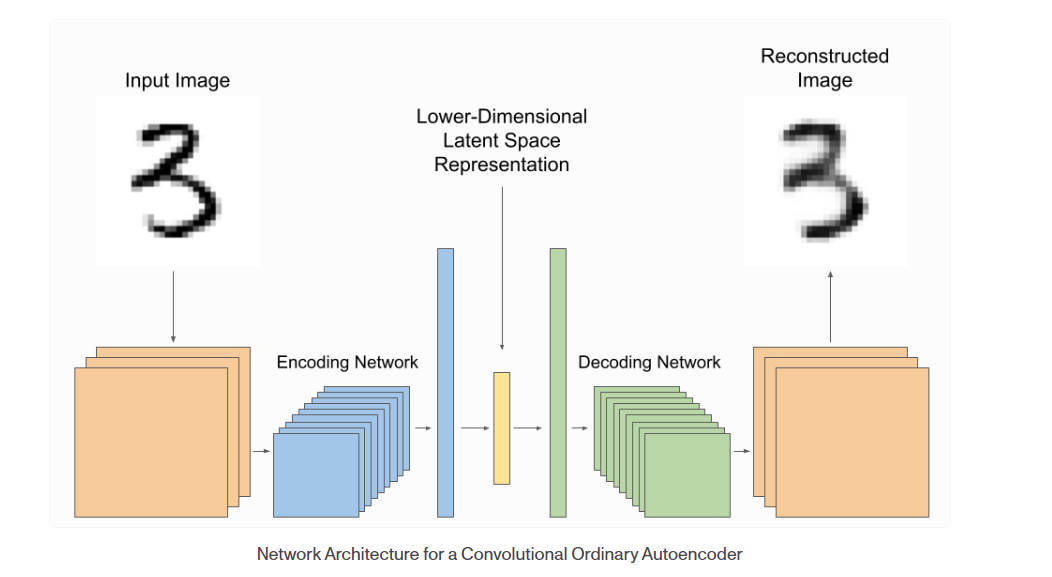
\includegraphics[width=90mm,scale=0.5]{images/autoencoder_images/assemblyai_reconstruction.png}

            \caption*{An example of the original vs reconstructed image from MNIST. Credit to \href{https://www.assemblyai.com/blog/introduction-to-variational-autoencoders-using-keras/}{assemblyai.com}}
        \end{figure}

        The reconstructed 3 above is still very recognizable, but it's clearly been "degraded" somewhat: it's not the same.

        \phantom{}

        

        \begin{clarification}
            
            The reconstructed input is usually \gren{not exactly the same} as the input.

            \begin{equation*}
                x \neq \tilde{x}
            \end{equation*}

            Our re-construction is an \orgg{approximation}.
        \end{clarification}

        We're essentially running our input through a "\vocab{bottleneck}", in a lower dimension.

        \begin{itemize}
            \item We do so, hoping that the right compression size "squeezes out" only unnecessary information.\\
        \end{itemize}

        \begin{concept}
            An autoencoder is, technically, just a normal neural network, where:

            \begin{itemize}
                \item We want the \gren{input} to equal the \gren{output} (re-constructed input)
                \item We monitor an \purp{intermediate layer} (latent representation), where the layer output size ($k$) \redd{decreases} below the input size ($d$)
                \item If our input and output match well enough, then we use the \orgg{output} of that \purp{intermediate layer}.
            \end{itemize}
        \end{concept}


\pagebreak
\section{Autoencoder Learning}

    Now that we've defined our autoencoder, it's time to \textbf{train} it.

    What's our objective? Well, we want to create a lower-dimensional representation that can be used to \textbf{re-construct} the original.

    \begin{itemize}
        \item We've handled the lower-dim aspect with the \textbf{structure} of the neural network: the last layer of the \gren{encoder} will output $k$ values, giving our \textbf{latent representation}.
            \note{Where $k<d$, given $d$ is the original input dimension.}
        \item So now, we need to show that this representation contains the information we want: it's able to \textbf{re-construct} the original.
            \begin{itemize}
                \item This is the job of the \purp{decoder}.
            \end{itemize}
    \end{itemize}

    That latter point is what we need to address: we need to check the quality of our re-construction, $\tilde{x}$.\\

    \begin{concept}
        We measure the \orgg{quality} of our autoencoder by measuring the \gren{similarity} between the original input $x$, and the re-constructed input $\tilde{x}$.

        \begin{itemize}
            \item If the re-construction is similar to the original input, that means our latent representation successfully \purp{encodes} information about $x$.
        \end{itemize}
    \end{concept}

    So, we need some kind of \textbf{similarity} metric. We'll encode this into our loss function, $\loss$. $\loss$ tells us how \textbf{different} our re-construction is, from the original.

    \begin{itemize}
        \item For \purp{continuous} variables, you might use \textbf{squared distance} between $x$ and $\tilde{x}$: loss $\loss_{SE}$.
            \note{"SE" stands for "squared error". It's different from MSE, "mean squared error", because we're not dividing by $d$.}

        \begin{equation}
            \loss_{SE} = \norm{x-\tilde{x}}^2 = \sum_{i=1}^d (x_i-\tilde{x}_i)^2
        \end{equation}
    \end{itemize}

    Note that often, an input does not only contain one data type: it may include different types of \textbf{discrete} data. 

    So, you may need to use different loss functions for different dimensions of the input.

    \subsecdiv

    Now that our problem is fully framed, we can simply \textbf{optimize} it, to minimize loss, using our parameters.\\

    \begin{concept}
        Once we've chosen our loss function, we can \gren{optimize} our autoencoder as an ordinary neural network, in order to create our \purp{encoder} for latent representations.

        \begin{itemize}
            \item $W_{en}$ and $W_{de}$ are our encoder and decoder weights, respectively.

        \end{itemize}

        Our goal is to optimize these weights, with respect to the \purp{loss}, over our $n$ data points:

        \begin{equation*}
            W_{en}^*, W_{de}^* =  \operatorname{argmin}_{W_{en}, W_{de}} 
            \Bigg( {\sum_{i=1}^n \loss(\red{\ex{\tilde{x}}{i}}, \blu{\ex{x}{i}})} \Bigg)
        \end{equation*}
        
        Or, if we want to be more explicit,

        \begin{equation*}
            W_{en}^*, W_{de}^* = \operatorname{argmin}_{W_{en}, W_{de}} 
            \Bigg( \sum_{i=1}^n 
            \loss( \red{NN(\ex{x}{i}; W_{en},W_{de})} ,\; \blu{\ex{x}{i}}) 
            \Bigg)
        \end{equation*}

        \subsecdiv

        \begin{itemize}
            \item As usual for neural networks, we often optimize using gradient descent via \purp{back-propagation}.
        \end{itemize}
    \end{concept}

        \note{Remember that $W^*$ notation is used to indicate "optimal" parameters.}

        \miniex For our one-layer encoder/decoder above, we would optimize over $W^1$, $W^1_0$, $W^2$, $W^2_0$.

    
\pagebreak
\section{Evaluating an Autoencoder}

    After \textbf{training} our autoencoder, we want to be able to \textbf{confirm} that it does what we want.

    What do we \textbf{want}?

    \begin{itemize}
        \item A representation that contains \textbf{fewer} dimensions than the input: $k < d$.
            \note{Often, a latent representation can be \textbf{much} smaller than the input.
            
            \phantom{}
            
            Remember our MNIST example at the start of the chapter, going from 784 dimensions, to 2.}

            \begin{itemize}
                \item Remember that $k$, in this case, is the dimension of our \textbf{latent} representation, and $d$ is the dimension of our \textbf{input}.
            \end{itemize}

        \item For this representation to contain useful \textbf{information} about our input.
            \begin{itemize}
                \item This second aspect is (hopefully) addressed by our \textbf{loss} function. 
                \item If our \textbf{re-constructions} are really good, then we've managed to preserve our information.
            \end{itemize}
    \end{itemize}

    \subsection{Dimensionality of $a$}

        Our loss function handles the latter of these two problems, but the \textbf{dimensionality} is based on our \textbf{choice} of NN structure.

        Well, if we're compressing our data, we want to reduce our number of dimensions, typically. But there's a tradeoff:\\

        \begin{concept}
            The \purp{smaller} our latent representation is, the \purp{less information} we can store in it.

            \begin{itemize}
                \item So, our re-constructions will be generally \purp{worse}.
            \end{itemize}

            But a \gren{larger} latent representation uses more \gren{space}/computation, and doesn't \gren{filter} out as much unnecessary, distracting information.
        \end{concept}

        \phantom{}

        \begin{clarification}
                Because we want to \purp{compress} our data, we require $k < d$. 

                If we allow $k=d$, then our "latent representation" could be the \gren{exact same} as our original representation.
                \begin{itemize}
                    \item In fact, that would be the most \gren{efficient} way to always be correct.
                    \item If $k>d$, then we have extra dimensions, prone to overfitting.
                \end{itemize}
    
                If we \redd{remove} the $k<d$ requirement, we're not forcing our network to do any real work, and our representation \redd{doesn't} have to become more efficient.
            \end{clarification}
    
            In short: if we're not making the dimensions smaller, then we're not really compressing our data!

            But what if we wanted to try making the dimensions \textbf{larger} on purpose? Does that have applications?\\

            \begin{concept}
                You might wonder if $k>d$ would let us "\purp{unpack}" some of our input data into those extra dimensions.
                
                An encoder with $k>d$ is called an \vocab{overcomplete autoencoder}.
                
                Usually, this is \textbf{not} desirable:
    
                \begin{itemize}
                    \item Our goal of "recreating the input" doesn't lend it itself well to "unpacking the data": it's usually easier to just \gren{copy} the input.
                    \item Moreover, \purp{overfitting} makes these autoencoders hard to train.
                \end{itemize}

                That said, this sort of approach does have applications in de-noising, and learning sparse representations.
            \end{concept}

            \subsecdiv

            Just like in clustering, your exact choice of latent dimensionality $k$ (usually $k < d$) is often subjective or task-based, and requires some trial and error.

            We might have different considerations:

            \begin{itemize}
                \item How well does the plot seem to organize our data?
                \item Are we missing some crucial kind of information?
                \item Have we encoded information we don't care about on accident?
            \end{itemize}

            And more.

    \subsection{Data Analysis}

        One of the reasons we wanted to design autoencoders was to learn more about our data.

        So, a useful encoder might be one that gives us some new or interesting insights.\\

        \begin{concept}
            We can learn more about our (already trained) encoding by \purp{experimenting} with it.

            How? By \purp{modifying} the latent representation $a$, and seeing how that affects the re-constructed version $\tilde{x}$.

            

            \begin{itemize}
                \item We could start with a known data point, and modify one \gren{dimension} of it, $a_j$. 
                \item If we increase $a_j$ and get a noticeable change, we can make guesses about what that dimension "\gren{represents}".
            \end{itemize}
        \end{concept}

        \miniex Suppose that we embedded the MNIST digits with $k$ dimensions.

        \begin{itemize}
            \item We select one random data point, $\ex{x}{i}$. This data point happens to be a picture of the number 6.
            \item We scale up/down one dimension, $a_j$.
            \item We might see that the line thickness of the 6 increases. Maybe $a_j$ represents line thickness.
        \end{itemize}

        There could be many possible features: how "angular" the number is, how it loops, etc.

        Not to say that those are the particular features you \textit{will} find. In fact, sometimes, it's totally unclear what your latent representation is "representing".

        \subsecdiv

        A few other examples of how to do our data analysis:\\

        \begin{concept}
            Rather than "experimenting" with individual axes, we could \purp{plot} data points in the \orgg{latent space}.

            There are two ways to do this:

            \begin{itemize}
                \item Take \purp{real} data points, and plot where they appear in the latent space, compared to how the \gren{input} looks.

                \item Directly \purp{sample} points from the latent space, and see what their \gren{re-construction} looks like.
            \end{itemize}

            In both cases, we get an idea of how the autoencoder interprets the data it receives.
        \end{concept}

        \miniex We started the chapter with an example of the former technique:

        \begin{figure}[H]
            \centering
            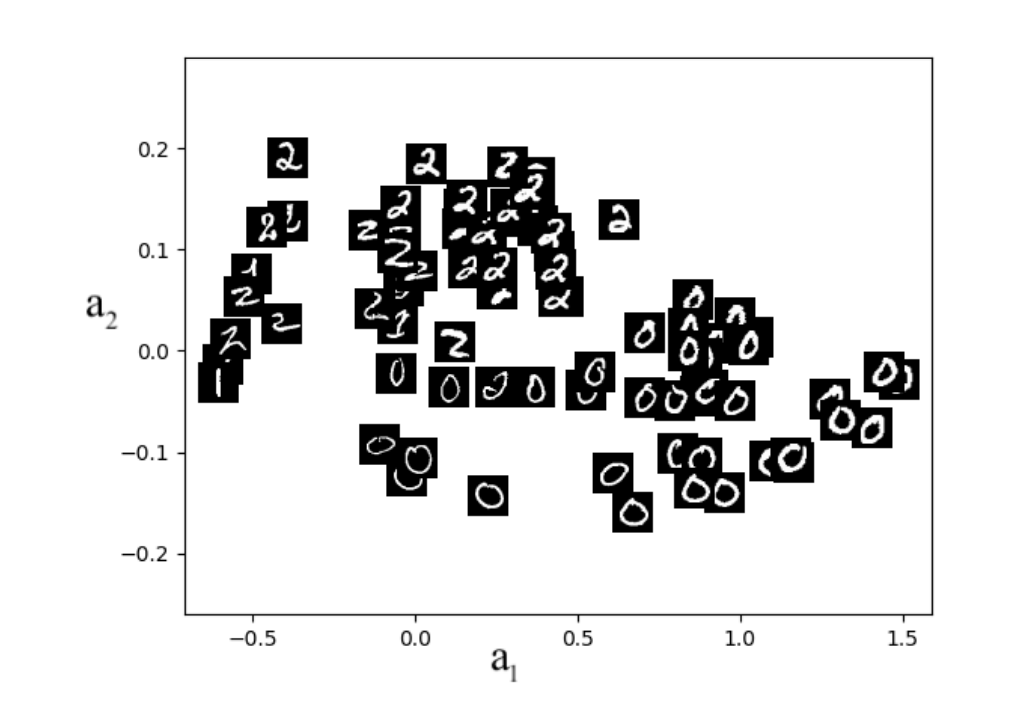
\includegraphics[width=70mm,scale=0.5]{images/autoencoder_images/mnist_compression.png}
            \caption*{Here, we take real data points, and plot them in the latent space.}
        \end{figure}

        \miniex We could also use the latter: seeing how our re-construction appears, as we modify our latent variables.

        \begin{figure}[H]
            \centering
            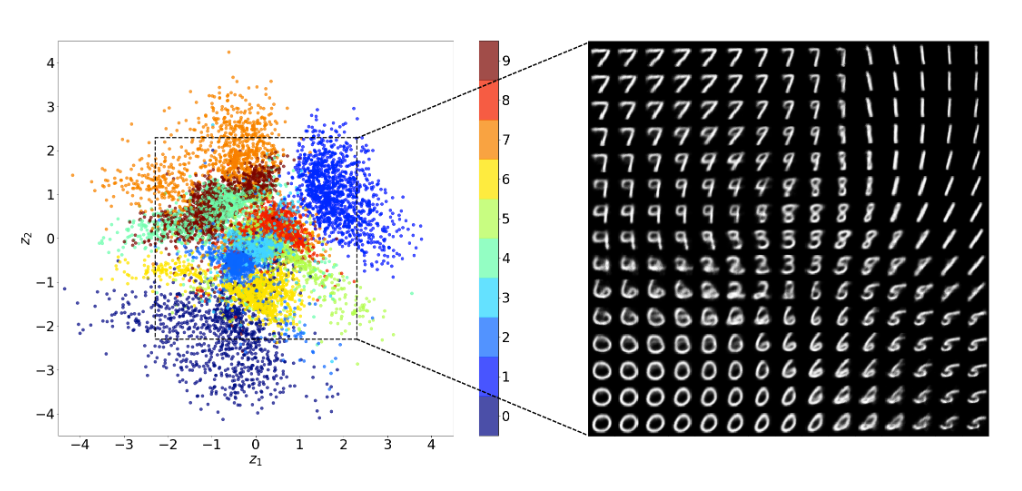
\includegraphics[width=90mm,scale=0.5]{images/autoencoder_images/latent_space.png}
            \caption*{The left shows the position of real digits in latent space, while the right shows our re-constructions, moving in a grid across the space. Credit to \href{https://argmax.ai/blog/vhp-vae/}{argmax.ai}.}
        \end{figure}

        \begin{concept}
            Lastly, we could see what the model thinks the data \purp{generally} looks like, based on the biases/offsets in the network.
                \begin{itemize}
                    \item The offset values ($W_0^\ell$) are the \gren{same}, regardless of the data point.
                    
                    \item We could set all of the values of $a$ to 0: in a \purp{linear} autoencoder, this would give the \purp{average} of our data points. 
                \end{itemize}

                \subsecdiv

            If our data clusters around the average, it would be reasonable to expect the average to be \gren{somewhat similar} to all of our data.

            \begin{itemize}
                \item And if it looks similar to each data point, it could somewhat \purp{represent} what it looks like in general.
            \end{itemize}

            In a \textbf{non-linear} autoencoder, our above approach doesn't give us the \textbf{average}, but could be useful regardless.
        \end{concept}


        After analyzing all our dimensions, we can try to figure out what \orgg{information} the encoding decided was "important", or at least, necessary for re-construction.

        This kind of analysis has a wide array of applications, including natural language processing, disease subtyping, and image processing.

    \subsection{Downstream Tasks}

        If we're using the encoder for downstream tasks, we can evaluate the autoencoder based on the performance of those downstream tasks.

        \begin{itemize}
            \item We mentioned the same kind of metric when we discussed clustering.\\
        \end{itemize}

        \begin{concept}
            Performance on \vocab{downstream tasks} is one way to evaluate the quality of an encoding.
        \end{concept}

        One simple approach, is to use \purp{semi-supervised learning}.\\

        \begin{definition}
            \vocab{Semi-supervised learning} provides labels for only \purp{some} of the data we use to train. The rest of it is unlabelled.

            So, the model has to \gren{extrapolate} from that data, to figure out a pattern for the rest of the data.
        \end{definition}

        If we have a \textbf{meaningful} latent representation, we could use it to help with this type of problem.

        \miniex We'll re-use our MNIST example. Suppose we were only given a \textbf{few} labelled digits:
            

        \begin{figure}[H]
            \centering
            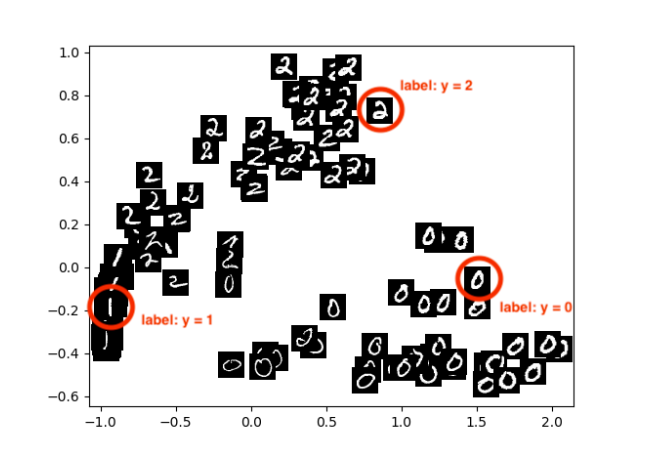
\includegraphics[width=70mm,scale=0.5]{images/autoencoder_images/semi_supervised.png}
            \caption*{Only the three labelled data points are "supervised".}
        \end{figure}

        \begin{itemize}
            \item In this case, we could label many of these digits, just based on what we have.
                \note{3 data points is a really small amount of information! This makes it even more impressive.}
        \end{itemize}

        The fact that this approach works so well, with only 2 dimensions, tells us that our encoding is impressively effective.

        

        

    \pagebreak

\section{Linear Encoders and Decoders}

    Even simpler than our one-layer example above, is the \textbf{linear} autoencoder.

    It turns out that, despite its simplicity, even a linear autoencoder can be useful! In some contexts, it's even \textbf{better}:

    \begin{itemize}
        \item A linear autoencoder often has a \textbf{closed-form} solution: we don't have to do gradient descent.
        \item The linear autoencoder tends to create a very simple kind of \textbf{interpretability}.
    \end{itemize}

    This closed form solution is equivalent to \vocab{principle component analysis} (PCA), which you might be familiar with from linear algebra.

    \begin{itemize}
        \item We obtain this solution using a technique called \vocab{singular value decomposition} (SVD).
    \end{itemize}

    \subsecdiv

    We can draw some parallels to a paradigm we've seen before:

    \begin{itemize}
        \item \gren{PCA} can be thought of as the simplified, linear version of the \purp{autoencoder} problem. 
        \item This is similar to how \gren{linear regression} is the simple, linear version of a \purp{neural network}.
    \end{itemize}

    \pagebreak

    \subsection{Principle Component Analysis (\red{Optional})}

        \phantom{}

        \begin{remark*}
            The following section briefly covers the concepts of PCA. 

            These may provide some intuition for what autoencoders do, in a simple, linear environment.
        \end{remark*}

        We mentioned that autoencoders need to make their data points clearly \textbf{distinct} from one another.

        \begin{itemize}
            \item In other words, it's best to focus on ways that they're \textbf{different} from each other.
        \end{itemize}

        The easiest way to do that is to focus on sources of \textbf{variance} in the data.

        \subsection{Low-variance: less important (\red{Optional})}

            Let's give a motivating example:

            \begin{figure}[H]
                \centering
                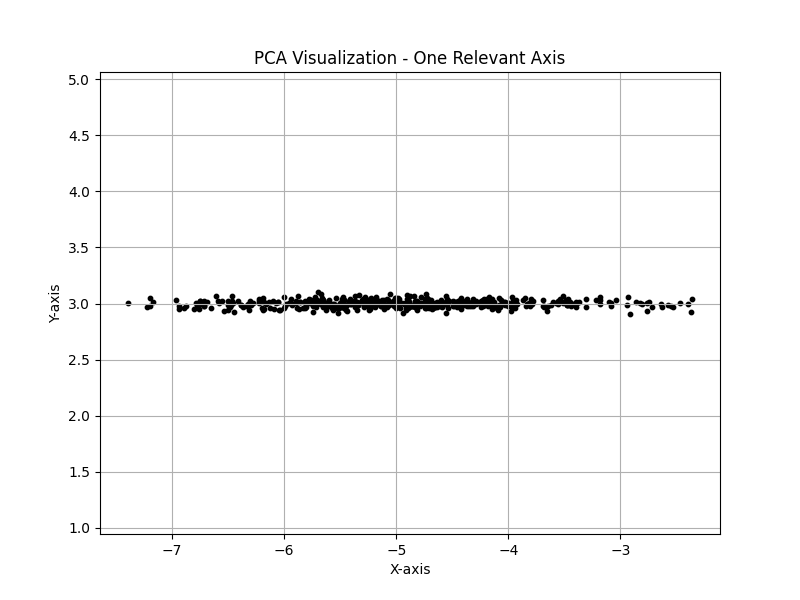
\includegraphics[width=70mm,scale=0.5]{images/autoencoder_images/pca_x_axis.png}
                \caption*{Almost all data is encoded on the $x$-axis.}
            \end{figure}

            If we look at this dataset, there's a clear \textbf{difference} between our two axes: one is very high-variance ($x$), one is low ($y$).

            If I told you "the $y$ coordinate of this data point is roughly 3", that tells you essentially \textbf{nothing}: that's true of all of our data.

            Meanwhile, the $x$ coordinate is much more \textbf{informative}.

            \begin{itemize}
                \item It seems that \textbf{high-variance} dimensions tend to contain \textbf{more information} than low-variance dimensions.
            \end{itemize}

            So, if we break our data up based on coordinates:

            \begin{figure}[H]
                \centering
                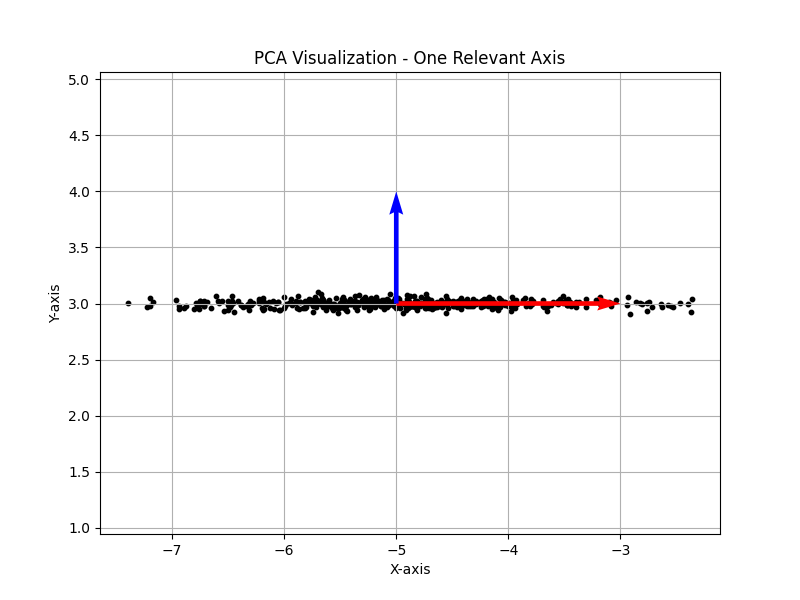
\includegraphics[width=70mm,scale=0.5]{images/autoencoder_images/pca_x_axis_vec.png}
            \end{figure}

            We could remove the $y$-axis while preserving most of our information! This would be a good target for \textbf{omitting} from the latent space.
            
            \begin{equation}
                \begin{bmatrix}
                    x \\ y
                \end{bmatrix}
                \longrightarrow
                \begin{bmatrix}
                    x
                \end{bmatrix}
            \end{equation}\\

            \begin{concept}
                When doing PCA, we tend to focus on axes of \gren{high variance}.

                Axes with low variance carry \purp{less information}.

                So, if we want to \vocab{compress} our data, we can remove those low-variance dimensions.
            \end{concept}

        \subsection{Different axes (\red{Optional})}

            Our data doesn't always (or even usually) line up perfectly with our axes, though.

            \begin{figure}[H]
                \centering
                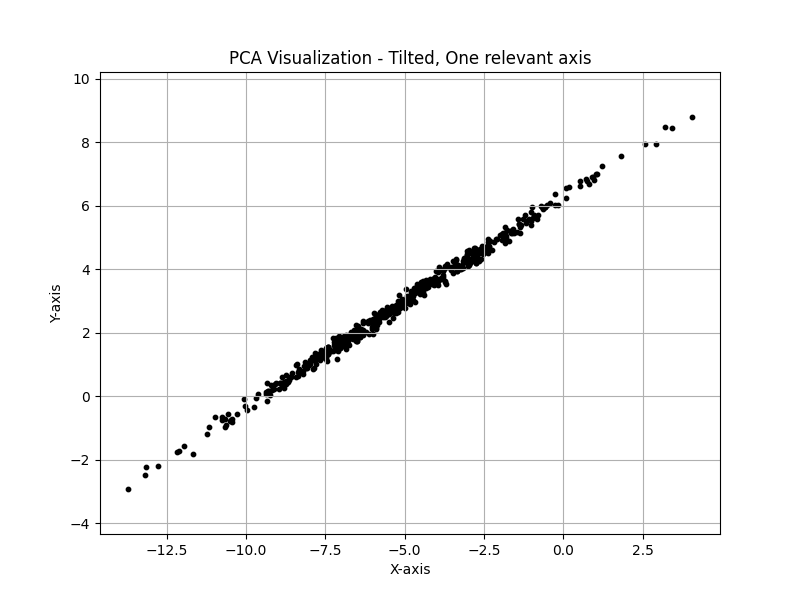
\includegraphics[width=70mm,scale=0.5]{images/autoencoder_images/pca_tilt_axis.png}
                \caption*{Almost all data is on a single line.}
            \end{figure}

            In this case, it looks very \textbf{similar} to our $x$-axis data. But the problem is, we can't just reduce it to one of our two axes.

            The solution? \textbf{Change coordinate systems}.

            \begin{figure}[H]
                \centering
                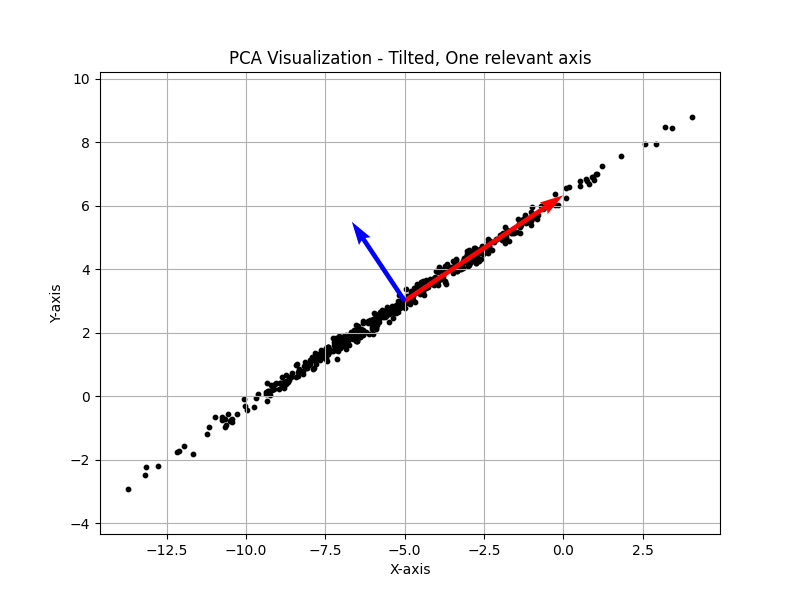
\includegraphics[width=70mm,scale=0.5]{images/autoencoder_images/pca_tilt_axis_vec.png}
                \caption*{Now, we have a high variance axis, and a low variance axis.}
            \end{figure}

            Now, we have the same situation as before! Almost all of our data is on \textbf{one axis}: we can omit the other.\\

            \begin{concept}
                Often, the most "\orgg{information}-heavy" directions in our data, aren't our default axes.

                So, we look for a \purp{new coordinate system}, where most of our variance is contained ("can be explained") by only a few dimensions.

                \begin{itemize}
                    \item That way, we can \redd{remove} the other remaining dimensions, which contribute very little to our understanding of the data.
                    \item With fewer dimensions, our data is often more \gren{interpretable}.
                \end{itemize}

                This idea, of finding high-variance components, and discarding low-variance components, is the core principle of \vocab{principle component analysis}.

                \begin{itemize}
                    \item This is equivalent to how our linear autoencoders remove extra dimensions.
                \end{itemize}
            \end{concept}

            Sometimes, it can be a bit difficult to \textbf{interpret} these high-variance components: what does it mean to have high variance along a "different axis", conceptually?

            But other times, we find that two "separate" variables, are both giving us the \textbf{same information}: they would correlate strongly, and thus, would give us the line we see above!

            \begin{itemize}
                \item This is why we can \textbf{remove} one dimension: we're using two axes to represent basically the same thing.
            \end{itemize}

            \miniex If something is sold for a fixed price, then "number of units sold" and "profits from sales" are telling us \gren{the same thing}.
                \note{Many examples aren't perfectly correlated like this, but are still pretty similar: for example, sales and advertising spending at a company.}

            So, we can compress into one dimension with low information loss.


    \subsection{General example (\red{Optional})}

        How many dimensions we need to capture most of our variance \textbf{depends} on the situation. 

        The goal is often, for visualization, to reduce it to \textbf{2 or 3} primary components.

        But even if we can't remove axes, PCA can give us a useful way to focus in on the \textbf{relationship} between our variables:

        \begin{figure}[H]
            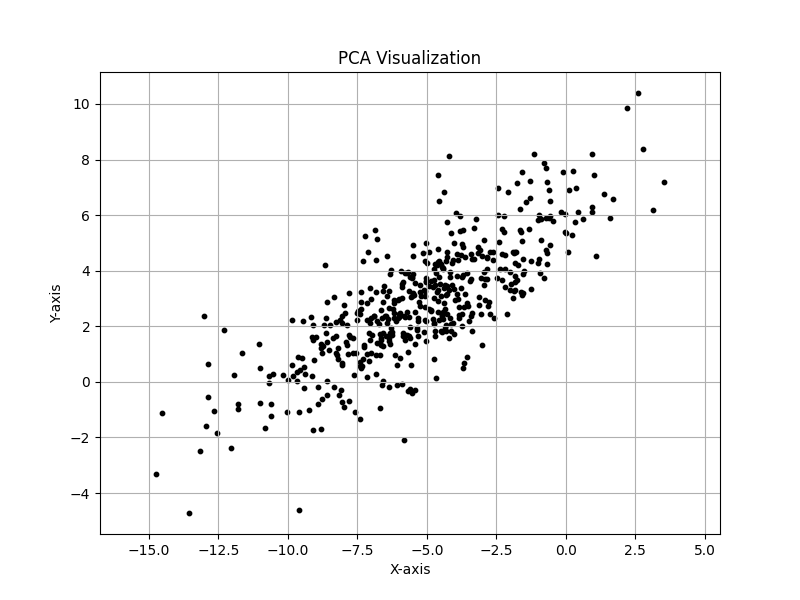
\includegraphics[width=70mm,scale=0.5]{images/autoencoder_images/pca_no_label.png}
            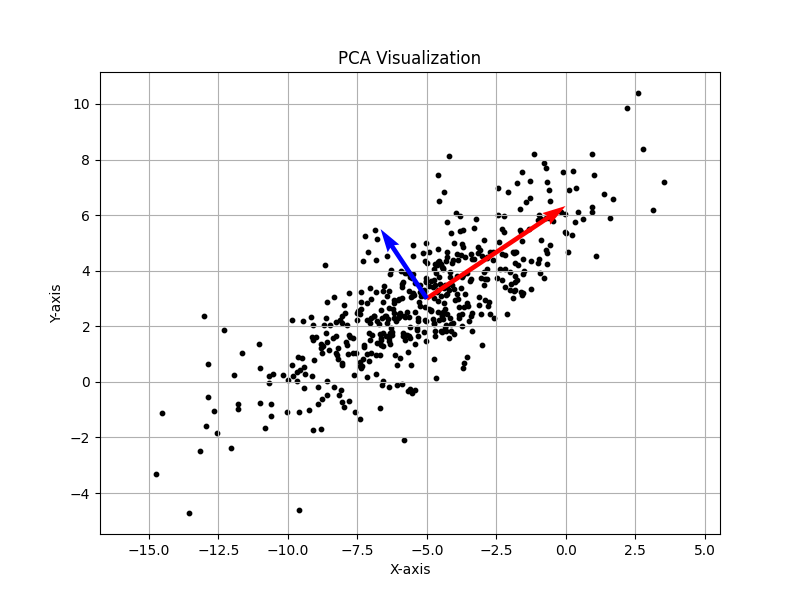
\includegraphics[width=70mm,scale=0.5]{images/autoencoder_images/pca_with_label.png}
            \caption*{Here, we have identified which axis matters "more" to our data, and how much.}
        \end{figure}

        

    \subsection{Non-linear encoders (\red{Optional})}

        Of course, things aren't always so simple: we often won't have this nice blob, which we can measure across a few perpendicular axes.

        Our real data might take on a different form, that has a coherent "shape", or "structure", but not one that fits our \textbf{linear} model.

        This is where our \textbf{non-linear} autoencoders come in. They follow the same kind of principles as PCA: 
        
        \begin{itemize}
            \item We want to distinguish patterns and curves that contain \textbf{variance}, and allow us to \textbf{distinguish} data points.
            \item Those which contain more information, we \textbf{keep}. The rest, we discard.
            \item We can then \textbf{visualize} those remaining dimensions, or use them for data analysis.
        \end{itemize}

        \subsecdiv

        One more detail of PCA we've ignored so far: all of variance comes from some "baseline": an \textbf{average} position, which all of our data points are \textbf{shifted} from.

        \begin{itemize}
            \item We could view this as a "\textbf{template}", which our PCA components point away from, for any given data point.
        \end{itemize}

        In PCA, we didn't focus on this as much, because it was just the average of all of our data points: useful, but simple.

        This concept becomes interesting in the more complex case of non-linear autoencoders: it isn't so easy to \textbf{guess} what's the "average"/typical example in the latent space.
        
        \begin{itemize}
            \item \miniex Suppose we plot all of the data points labeled "7", based on their latent representations.
            \item We could see what happens if we average those, and then convert it back into a picture: it would teach us about how our model sees the number $7$ in general.
                \note{The result depends on your exact choice of encoder, but it's not always what you expect: that's why it's so \textbf{informative}!}
            
        \end{itemize}

        
\pagebreak

\section{Advanced Encoders and Decoders (\red{Optional})}

    We can build on this framework to create models for different, practical tasks.

    \subsection{Generative Networks (\red{Optional})}

        One useful application of our latent space is to \textbf{artificially} create more data which is \textbf{similar} to the data we already have.

        How?

        We saw that, with \textbf{some} very effective autoencoders, we find some useful \textbf{structure} in our latent space:

        \begin{itemize}
            \item Data points which were \gren{nearby} in latent space, appeared \gren{similar} in the input space.
        \end{itemize}
        
        If we successfully train an autoencoder with this property, then creating new data is possible:
            \note{How do we train our autoencoder to do this? We'll discuss one popular approach below: the "variational autoencoder" (VAE).}

        \begin{itemize}
            \item We take our real data, and slightly modify it in the latent space. This should be similar to our real data, but not exactly the same.
        \end{itemize}
        
        This is the basis of a \textbf{generative network}:\\


        \begin{definition}
            \vocab{Generative networks} are networks which are used to \purp{generate} artificial data, which is similar to \textbf{real} data used to train it.

            These often come in the form of an autoencoder: 
            \begin{itemize}
                \item We start by using real data to \gren{train} the autoencoder, and create a \orgg{latent space}.
                \item We use those same data, and \gren{create} new data that is "close" to the real data, within our latent space.
                \item Finally, we use the decoder to \gren{reconstruct} our \purp{new data}.
            \end{itemize}

            \subsecdiv

            This technique relies on the assumption that data points which are \textbf{close} in the latent space, are \textbf{similar} in the input space.
        \end{definition}

        These models have many applications:

        \begin{itemize}
            \item Augmenting (increasing the size of) \textbf{smaller} datasets 
            \item Reducing \textbf{overfitting}, by perturbing data
            \item Art and Media
                \begin{itemize}
                    \item \miniex Superresolution: filling in "details" in images where they need to be believable, not necessarily real
                \note{This, of course, can cause problems if you don't know you're working with fictional data!}
                \end{itemize}
            
        \end{itemize}

        And more, which we'll discuss below.

        \subsubsection{Variational Autoencoders (\red{Optional})}

            We've introduced the general outline of a \vocab{generative network}: we create artificial data, using our latent space.

            But we have \textbf{two problems}:

            \begin{itemize}
                \item First: how do we \textbf{generate} \orgg{new} data points, "close" to the real data? What's our procedure? 
                
                \item Second: this relies on the assumption that our \textbf{encoding} is \gren{smooth}: nearby points in latent space represent similar information. How do we guarantee that?
            \end{itemize}

            We'll find that one technique addresses both of these problems: representing our data as a \textbf{probability distribution}.
            
            \subsecdiv

            One simple way to generate new data, is to \purp{randomly} perturb a data point in the latent space, by a small amount.

            The outcomes of random processes, like this, have a certain \textbf{probability} of occurring.
                \begin{itemize}
                    \item So, the output of our encoder isn't a point in the latent space, but a \purp{probability distribution} of possible points.\\
                \end{itemize}

            \begin{definition}
                A \vocab{variational autoencoder}, rather than creating a \gren{single} encoding for a data point, encodes a \purp{probability distribution}.

                \begin{itemize}
                    \item This distribution represents different possible encodings, for the \gren{same} input.
                \end{itemize}

                Then, we \orgg{sample} from this distribution, to randomly select an encoding.

                Finally, we \textbf{decode} this to get our "modified" data point.

                \subsecdiv

                \item This process actually \orgg{regularizes} our model: it needs to be able to re-produce the input, even if it's slightly modified in the latent space.

                \begin{itemize}
                    \item We're also restricting our probability distribution to have a certain shape/structure (like a normal distribution).
                \end{itemize}
                
            \end{definition}

            \miniex Suppose that we created a 1-D encoding, and for this particular data point, we encode it as $a=2$. If we compare the simple AE to the VAE:

            \begin{figure}[H]
                \centering
                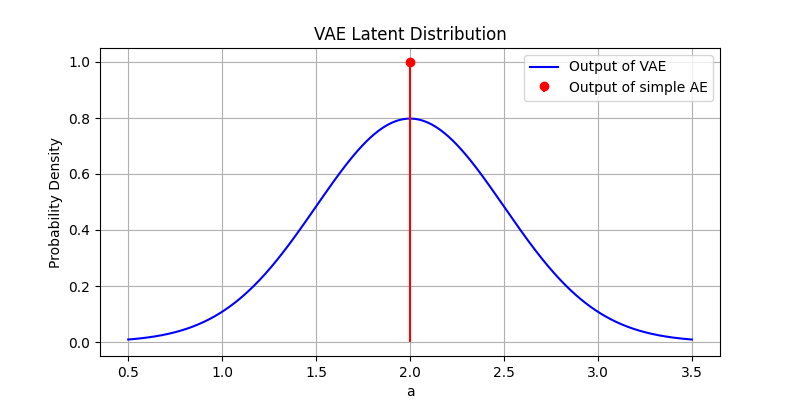
\includegraphics[width=90mm,scale=0.5]{images/autoencoder_images/vae_latent_distribution.png}
                \caption*{We've gone from "always output 2" to "output a normal distribution centered on 2".}
            \end{figure}
                \note{Technical comment, that isn't important to this class:
                
                \phantom{}
                
                The simple AE distribution depicted is the \textbf{dirac delta function}, where all the probability is 'stored' at $a=2$.}

            We can directly compare the process in both cases. First, the \vocab{simple autoencoder}:

            \begin{equation}
                x  \quad \xrightarrow[encoding]{} \quad
                \org{a=e(x)} \quad \xrightarrow[decoding]{} \quad
                \tilde{x} = d(a)
            \end{equation}

            Next, the \vocab{variational autoencoder}:

            \begin{equation*}
                x  \quad \xrightarrow[encoding]{}
                \overbrace{ \org{p(a|x)} }^{\text{Distribution}}
                \xrightarrow[sampling]{}
                \overbrace{ \org{a \sim p(a|x)} }^{\text{$a$ sampled from $p(a|x)$}}
                \xrightarrow[decoding]{} \quad
                \tilde{x} = d(a)
            \end{equation*}

            \subsecdiv

            Now, we can handle the second problem: how do we ensure that nearby points in the latent space are \gren{similar}?

            Well, if we want our model to do something, we \orgg{train} it with that goal in mind.

            \begin{itemize}
                \item As we've designed it, our VAE \textbf{already} generates points "nearby" to our encoding, using its probability distribution.
                    \note{We usually use something like the normal distribution above: most data is close to the mean.}

                \item Because they're nearby, we want the \textbf{original} data and the \textbf{sampled} data to be relatively similar.\\
            \end{itemize}

            \begin{concept}
                Unlike a simple AE, our VAE \redd{doesn't} return exactly the same data that it started with: 

                \begin{itemize}
                    \item Instead, our VAE \purp{samples} the latent space, \gren{nearby} to the "pure" encoding.
                \end{itemize}

                Because the sampled and original data are nearby, we want them to be \gren{similar}.
            \end{concept}
            
            How do we compare the original and sampled data? The original data is given as the input. Meanwhile, we convert the sampled data by \textbf{decoding} (reconstructing) it.

            We want our original (input) data $x$ and sampled (+decoded) data $\tilde{x}$ to be \textbf{similar}. 
            
            \begin{itemize}
                \item This is similar to our goal for the simple autoencoder: there, too, we wanted our original and re-constructed data to match.\\
            \end{itemize}

            \begin{concept}
                Just like with a simple autoencoder, we want the \gren{input} and \purp{output} of our VAE to be close to \textbf{equal}.

                \begin{equation*}
                    x \approx \tilde{x}
                \end{equation*}

                This serves a few functions:

                \begin{itemize}
                    \item Same goal as we had before: being able to \purp{reconstruct} the input shows that our encoding preserves meaningful \textbf{information}.

                    \item The simple encoding of $x$, and the encoding that produces $\tilde{x}$, are \textbf{not} the same, but they are \gren{similar}.
                        \begin{itemize}
                            \item This helps us train our model to "\purp{smooth out}" its surface: we teach it that nearby points should be similar.
                        \end{itemize}
                \end{itemize}

                So, we \orgg{train} our model with this goal in mind.

                \subsecdiv

                To help "smooth out" the VAE representation further, we often add a \textbf{regularizer} term to the loss.

                \begin{itemize}
                    \item We won't go into detail on this feature here.
                \end{itemize}
            \end{concept}
            

    \pagebreak


            

            

    \subsection{Adversarial Optimization (\red{Optional})}

        We'll make a brief detour, to discuss a different way we can generate \orgg{artificial} data.

        In order to "test" your network, and see how \textbf{robust} it is, you might want to deliberately find examples it \orgg{struggles} with, but \textit{shouldn't}.

        \begin{itemize}
            \item We could do this by just running a large amount of data, and manually looking for examples that fail, despite seeming "obvious" to humans.
            \item But this is labor-intensive, and \purp{expensive}.
        \end{itemize}

        Instead, we introduce a different way to create so-called "\vocab{adversaries}": examples specifically designed to "trick" our model.

        We want a data point that:

        \begin{itemize}
            \item \gren{Should} be classified correctly, and would be classified correctly by humans
            \item But the machine fails, despite looking \purp{similar} to valid data points.
        \end{itemize}

        \subsecdiv

        We'll start with a valid, \textbf{correctly} labelled data point: this handles the first condition: "should have been labelled correctly".

        But we want to \textbf{modify} it so that it's labelled incorrectly.
        
        \begin{itemize}
            \item If our model isn't \textbf{robust} enough, we might be able to \textbf{confuse} it, without changing the data very much at all.
        \end{itemize}

        How do we modify it most efficiently? Using the \textbf{gradient}.

        Previously, we used the gradient to compute, "what's the most efficient way to change my \purp{model}, to \gren{decrease} my loss?"

        \begin{equation}
            W - \eta \pderiv{L}{W}
        \end{equation}

        This time, we want to ask, "what's the most efficient way to change my \purp{data point}, to \gren{increase} my loss?"

        So, we want the gradient between the loss and the data point.

        \begin{equation}
            x + \eta \pderiv{L}{x}
        \end{equation}

        We take \textbf{steps} in this process, repeatedly changing our gradient to match the model.
            \note{This time, instead of traveling across the parameter space, we're traveling across the input space!}

        We continue this process until our data point is successfully classified \textbf{incorrectly}.

        \begin{itemize}
            \item Often, we can accomplish this without significantly modifying our data point.\\
        \end{itemize}

        \begin{definition}
            \vocab{Adversarial training} is a way to "trick" a model into making inaccurate predictions:
            
            This is done by \gren{training} data points that appear very similar to real data, but exploit weaknesses of the model.

            \subsecdiv

            To accomplish this, we take a real, correctly labelled data point, and slowly apply gradient descent \orgg{to the data point}, gradually increasing the loss:

            \begin{equation*}
                x_{new} = x_{old} + \eta \pderiv{L}{x}
            \end{equation*}

            With some training, we can design a new data point that our model evaluates incorrectly, despite being very similar to the original data point.
        \end{definition}

            \miniex Here's a \textit{real example} of applying this to image classification:

            \begin{figure}[H]
                \centering
                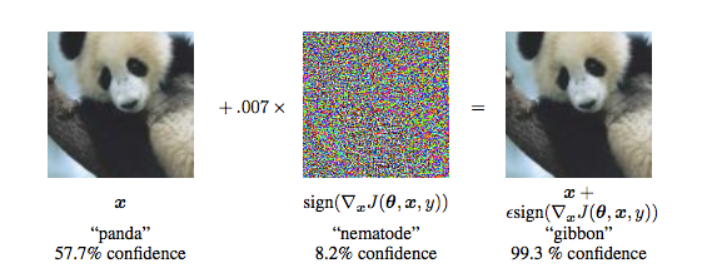
\includegraphics[width=80mm,scale=0.5]{images/autoencoder_images/panda.png}
                \caption*{This panda, despite no visible change in appearance, is now a gibbon. (Source: Ian Goodfellow et al., 2014}
            \end{figure}

        This kind of data is actually incredibly valuable: 
        
        \begin{itemize}
            \item If we use it to train our model further (i.e., teaching it that it's wrong about these data points), it tends to become \textbf{more robust} against this kind of attack.
        \end{itemize}

        But, we need to be careful in this process:\\

        \begin{clarification}
            When creating adversarial data, we have to set a \redd{termination} condition:

            If we continue gradient descent too long, our data point will change \gren{classification}, but it can also actually change enough that it \purp{should} be identified differently.
        \end{clarification}

        \miniex If you do gradient descent to turn a picture of a "9" into a "1", and it looks like a "1" to a human, it should be reasonable that the model makes the same decision.

        We want to find the point where the data is different enough to be deceptive, but not different enough that it's obviously, genuinely a new data point.

        Adversarial data is widely useful:

        \begin{itemize}
            \item Improving model robustness
            \item Defending against security threats
            \item Learning more about the nature of your model
        \end{itemize}


    \subsection{Generative Adversarial Networks (\red{Optional})}

        We've developed two useful ideas:

        \begin{itemize}
            \item Generative networks: used to generate artificial, plausible data
            \item Adversarial data: data designed to exploit weaknesses in a model
        \end{itemize}

        We can combine these ideas to create a powerful tool, called, appropriately, a \vocab{Generative Adversarial Network}.

        Here's the general idea:

        \begin{itemize}
            \item \purp{Generators}: we want to generate artificial data, that closely reflects the \gren{original} distribution. 
            
            \item We found that an \purp{adversary} could teach us (and in turn, our models), their weaknesses, by actively seeking them out.

            \begin{itemize}
                \item So, we'll create an \textbf{adversary} for the generator: the \vocab{discriminator}. This punishes our model for creating data that is "detectably different" from real data. 
            \end{itemize}
            
            
        \end{itemize}

        The generator will create "adversarial data": this data is designed to \orgg{trick} the discriminator into thinking it's real.

        The discriminator will try to learn how to tell the two apart, and provide feedback to the generator, telling us how it made a mistake the previous time.

        This feedback loop gradually improves how "realistic" our data generated is, through a form of \vocab{unsupervised } learning.
            \note{The two models are "supervising" each other!}\\


        \begin{definition}
            A \vocab{Generative Adversarial Network} is a model that comes into two opposing, or "adversarial", parts:

            \begin{itemize}
                \item The \gren{generator} is trained to create "fake" data, that looks as plausible and realistic as possible.

                \item The \purp{discriminator} is trained to detect fake data
            \end{itemize}

            When one of these models fails, they teach the other model what they did wrong, to improve. 

            \begin{itemize}
                \item This process repeats until the discriminator accuracy reaches 50\%: if it's equally likely to mix up real/fake data, our generator has become indistinguishable from real data.
            \end{itemize}
        \end{definition}

        This is a sort of "arms race" between the two halves of our model.\\ 

        \begin{clarification}
            Why is best performance for the generator at \purp{50\%}?

            If it was 100\%, then the model always assumes the generator is real, and the real data is fake.

            \begin{itemize}
                \item But that's not true: the real data is \textit{also} real. The discriminator isn't doing its job correctly anymore.
            \end{itemize}

            Another perspective: if you knew your discriminator was always \redd{wrong}, then you could easily create a discriminator that was always right: just do the opposite of what you got before.

            \subsecdiv

            In short: 50\% is the best you can do, because your discriminator is completely \textbf{unsure} of its answer: which is what it really means to be "\orgg{indistinguishable}".
        \end{clarification}
        

        GANs have been high successful: this procedure not only improves robustness, but often creates a generally improved model. 

        They're useful for creating very effective generators of new data, and have been particular useful in the past for image generation.
            \note{GANs are still relevant, but if you want a more \textbf{modern} approach, you could look into \textbf{Diffusion} models, like Stable Diffusion.}

    \pagebreak

    \subsection{De-noising (\red{Optional})}

        One useful application of autoencoders is \textbf{de-noising}.

        \begin{itemize}
            \item We want to turn a noisy input into a less-noisy input.
        \end{itemize}

        \begin{figure}[H]
            \centering
            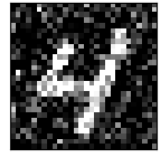
\includegraphics[width=30mm,scale=0.5]{images/autoencoder_images/noisy_4.png}
            \;\;
            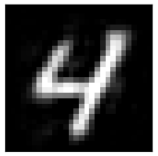
\includegraphics[width=30mm,scale=0.5]
            {images/autoencoder_images/clean_4.png}
            \caption*{The left is our input, right our desired, cleaner output.}
        \end{figure}

        The process for creating this kind of autoencoder is straightforward enough: we give noisy data and encourage the model to match the original, noiseless version.\\

        \begin{concept}
            Autoencoders can be used for \vocab{de-noising}:

            By training with 

            \begin{itemize}
                \item Noisy data as input
                \item Noiseless data as desired output
            \end{itemize}

            You can teach the model to create a latent representation that's resistant to this kind of noise.
        \end{concept}

    \pagebreak

    \subsection{Attention (\red{Optional})}

        Transformer networks are a very modern, very powerful approach to many problems, most famously \gren{language processing}.
            \note{As of writing, GPT-4 is the most famous example.}

        In order to create detailed context within a sentence, these models use a technique called "\vocab{self-attention}", which has proven to be incredibly powerful for working with language.

        \begin{itemize}
            \item Attention is an in-depth topic that deserves its own section; we'll \redd{skip} the math.
            \item The main idea: attention helps determine how words create \purp{context} for each other.
                \note{Transformers aren't \textbf{limited} to language, but we'll focus on that use case, for ease of explanation.}\\
        \end{itemize}

        \begin{concept}
            \vocab{Attention}, at a very high level, is based on the idea that:

            \begin{itemize}
                \item Different \gren{words} in a sentence have different levels of \purp{importance} to each other.
            \end{itemize}

            The words that are more \orgg{important} to a particular word $X$, are a bigger part of the \orgg{context} you use to understand that word.

            With that in mind, you can apply the \purp{context} from each other word $Y$, to better understand the meaning of word $X$.
        \end{concept}

        \miniex "The \vocab{blue dog} bites the \redd{red ball}": the word '\redd{red}' is describing the '\redd{ball}', so it is \textbf{less} important for understanding '\vocab{dog}' in this sentence.

        Based on that...\\

        \begin{definition}
            \vocab{Attention} is a mechanism for determining how, for a \purp{pair of words}, one word $X$ might might be \orgg{important} to understanding the other word $Y$, contextually.

            In other words, $X$ might require your \textbf{attention}, if you want to understand $Y$.

            \begin{itemize}
                \item Attention is applied to \purp{every} pair of words in a sentence: we measure every word's impact on every other word.
                \item Finally, for each word, we \gren{integrate} information from the other words, based on how "important" they were.
            \end{itemize}

            \subsecdiv

            Attention has the benefit of allowing us to analyze our entire prompt simultaneously, speeding up the process.
        \end{definition}

        Self-attention is used by a single sequence of text, by itself: it "learns about" itself.\\

        \begin{clarification}

            A few lingering comments:
        
            \begin{itemize}
                \item Word $X$ and $Y$ are typically asymmetric: $X$ may not affect the meaning of $Y$ the same way as $Y$ affects $X$.
                \item This meaning is \textbf{contextual}, not the "importance" of each word in isolation.
                \item We "integrate information" by taking a linear combination of each word: a larger weight is given to words which are more "important" to word $Y$.
            \end{itemize}
        \end{clarification}

        "Multi-headed attention" simply refers to having several of these attention mechanisms, applied to the same input in parallel.
            \note{So, each "attention head" receives the same data, like neurons in the same layer of a network.}

    \subsection{Transformer Networks (\redd{Optional})}

        Now that we loosely understand attention, we can think about the bigger picture.

        The goal of a transformer is to \purp{predict text}.

        At a very high level, transformers have a structure \textit{similar} to \gren{autoencoders}. They're broken into the same sort of two parts, though their internal structure is a bit \textbf{different}:

        \begin{itemize}
            \item \gren{Encoder}: this is actually a \textbf{stack} of several encoders, one after another. This (presumably) creates an \orgg{internal representation} of the "meaning" of the input text, similar to a latent representation.
                \note{You could say that this converts the input "prompt" into something similar to the "latent representation", which retains our key information.}
            
            \begin{itemize}
                \item Each encoder contains a fully connected network, as we've shown above, but also a "self-attention mechanism".
            \end{itemize}

            \item \purp{Decoder}: a stack of decoders, one after another. Based on the \orgg{internal representation}, it creates  predicted text.
                \note{This would create the "response" to your "prompt".}
                \begin{itemize}
                    \item Each decoder also contains an FC network+attention mechanisms.
                    \item Once our decoder predicts some text, that's part of the "\gren{past text}": this gets included alongside the internal representation, for future predictions.\\
                \end{itemize}
        \end{itemize}

        \begin{concept}
            A transformer network follows a structure with some similarities to auto-encoders: using an \textbf{internal representation}.
            
            \begin{itemize}
                \item Converting its \gren{input} (prior text) into an \redd{internal representation}, similar to a latent representation.
                \item Converting that \redd{representation} into an \purp{output} (predicted text)
            \end{itemize}

            However, there are key differences:
            \begin{itemize}
                \item As the output creates new text, that is \orgg{included} with the internal representation.

                \item Our "predicted text" will \gren{not} be the \gren{same} as our past text.
            \end{itemize}
        \end{concept}

        Why multiple encoders?\\

        \begin{concept}
            The \purp{multiple} encoders are used to gradually find "more \gren{complex}" patterns (or concepts), as we move through more layers.

            \subsecdiv

            \begin{itemize}
                \item The idea is that, the first encoder combines words to finds \gren{basic}, simple language structures. 
                \item The second encoder has access to these simple structures, and can \purp{combine} them together to create a more complex structure.
                \item Each encoder is combining the results of the \textbf{previous} layer, to create something more complex.
            \end{itemize}

            
        \end{concept}

        This is similar to the structure and motivation behind \textbf{convolutional neural networks}, which we will cover later.\\

        \begin{definition}
            A \vocab{transformer network} is a model made of encoders and decoders that use \purp{attention} to determine the \textbf{structure} and \textbf{context} of the input "prompt", and create an output "response".


            The structure of a transformer network is:
            
            \begin{itemize}
                \item Several "layers" of \gren{encoders}, that take the input and interpret it, creating the internal representation
                \item An \orgg{internal representation} of the input, and the previous output of the decoder
                \item Several "layers" of \purp{decoders} that turn this representation+output, into more \purp{predicted text}
            \end{itemize}

            Predicted text is given as a \textbf{probability distribution}, using softmax.

            \begin{itemize}
                \item We select an element from this probability distribution before moving on to the next word.
            \end{itemize}
        \end{definition}

        We've skipped over many important details of transformers, but this gives us the gist.
            \note{In particular, we've skipped some components, like normalization layers.}\\

        \begin{clarification}
            A few key differences between an autoencoder and transformer networks:

            \begin{itemize}
                \item The input and output are the same in an autoencoder.
                \item Transformers use attention mechanisms.
                \item The internal representation in an autoencoder ("latent representation") is \textbf{smaller} than the input or output.
                \item They serve different purposes.
            \end{itemize}
        \end{clarification}

        \begin{figure}[H]
            \centering
            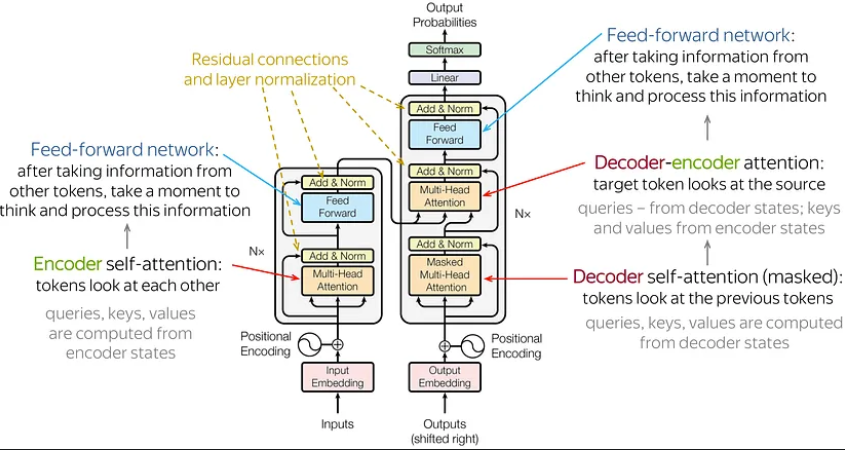
\includegraphics[width=100mm,scale=0.5]{images/autoencoder_images/transformers.png}
            \caption*{If you want a more in-depth explanation, go to \href{https://lena-voita.github.io/nlp_course/seq2seq_and_attention.html}{this very helpful resource}, and the source of this lovely diagram!}
        \end{figure}
        

\section{Terms}

    \begin{itemize}
        \item Unsupervised Learning (Review)
        \item Clustering (Review)
        \item Compression
        \item Decompression/Re-construction
        \item Encoder
        \item Decoder 
        \item Autoencoder
        \item Latent Representation
        \item Latent Space
        \item Bottleneck
        \item Dimensionality (Review)
        \item Overcomplete Autoencoder
        \item Downstream Task (Review)
        \item Semi-supervised Learning 
        \item Principle Component Analysis
        \item Singular Value Decomposition
        \item Generative Networks
        \item Variational Autoencoders
        \item Transformer Networks
    \end{itemize}

    \subsection*{\redd{Optional}}

    \begin{itemize}
        \item Adversarial Data
        \item Generative Adversarial Networks
        \item De-noising
        \item Attention
        \item Transformer Networks
        \item Internal Representation
    \end{itemize}

        

        
